\section{User Interface Design and Prototyping}

Building upon the established solution architecture and technical specifications, the design phase focused on creating an intuitive and professional user interface for Credix that addresses the usability shortcomings identified in existing solutions. The design process utilized Figma as the primary design tool to develop comprehensive mockups and interactive prototypes for the end-user mobile application.

\subsection{Design Approach and Rationale}

The UI/UX design of Credix directly addresses the critical usability issues observed in competing solutions, particularly the poor interface design and non-intuitive navigation found in Pluxee Tunisia and limited functionality in other payment applications. For a financial application like Credix, exceptional design is not merely aesthetic—it is essential for user trust, transaction security, and operational efficiency.

In retail payment systems, users often operate under time pressure during checkout processes. A well-designed interface reduces transaction time, minimizes user errors, and enhances the overall payment experience for both end-users and vendors. Poor design, as evidenced in existing solutions, leads to abandoned transactions, user frustration, and reduced adoption rates.

\subsection{Figma Implementation and Design System}

The design process established a comprehensive design system in Figma, incorporating modern UI/UX principles while addressing the specific requirements of the Credix ecosystem. The design system ensures consistency across all user interfaces through a carefully selected color palette featuring soft, professional tones with distinctive yellow accent colors for primary actions and navigation elements.

Key design decisions were made to differentiate Credix from existing solutions: streamlined navigation flows, clear visual hierarchy for transaction information, and intuitive iconography that reduces the learning curve for new users. The interface employs a clean, minimalist approach with ample white space and consistent typography to enhance readability and user confidence.

\subsection{Interface Design Showcase}

The following figures present the key interface designs developed for the Credix end-user mobile application, showcasing the user-centered approach and modern design principles implemented throughout the system.

\begin{figure}[H]
    \centering
    \begin{subfigure}[b]{0.32\textwidth}
        \centering
        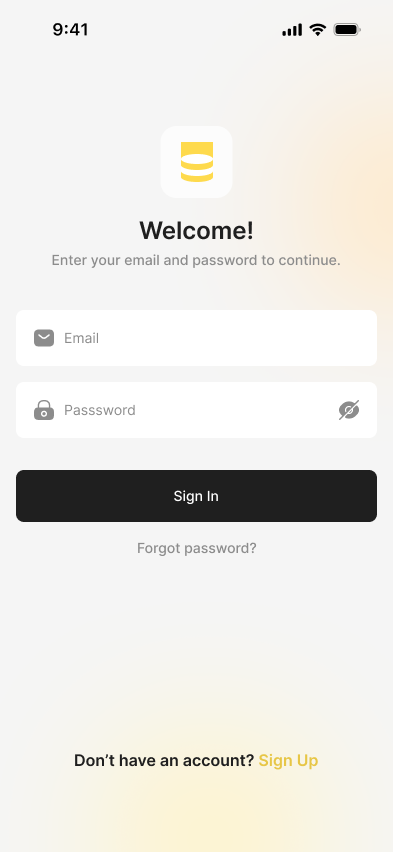
\includegraphics[width=\textwidth]{images/sign_in_screen.png}
        \caption{Sign In Screen}
        \label{fig:signin_screen}
    \end{subfigure}
    \hfill
    \begin{subfigure}[b]{0.32\textwidth}
        \centering
        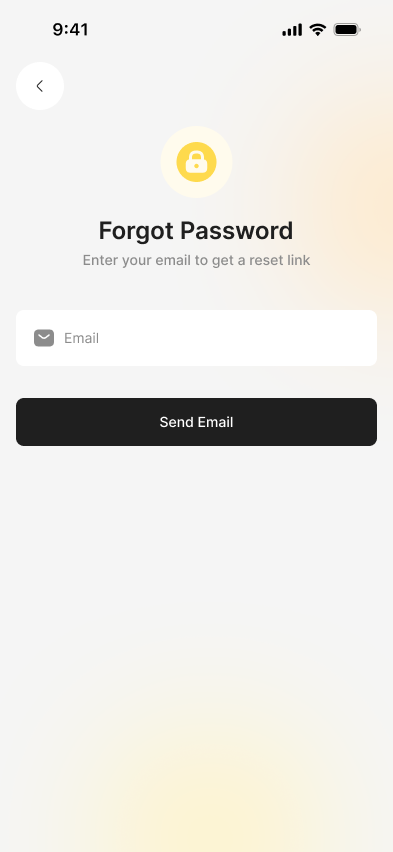
\includegraphics[width=\textwidth]{images/forgot_password_screen.png}
        \caption{Forgot Password Screen}
        \label{fig:forgot_password_screen}
    \end{subfigure}
    \hfill
    \begin{subfigure}[b]{0.32\textwidth}
        \centering
        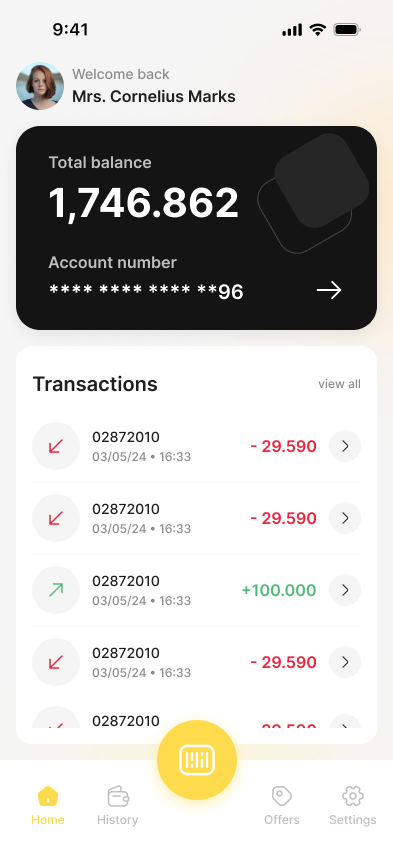
\includegraphics[width=\textwidth]{images/home_screen.png}
        \caption{Home Screen}
        \label{fig:home_screen}
    \end{subfigure}
    \caption{Authentication and Main Dashboard Interfaces}
    \label{fig:auth_dashboard}
\end{figure}

The authentication flow demonstrates a streamlined user experience with clear visual hierarchy and minimal cognitive load. The Sign In Screen features clean input fields with appropriate validation, while the Forgot Password Screen provides a straightforward recovery process. The Home Screen serves as the central hub, displaying account balance, recent transactions, and intuitive navigation—addressing the cluttered interface issues found in Pluxee Tunisia.

\begin{figure}[H]
    \centering
    \begin{subfigure}[b]{0.32\textwidth}
        \centering
        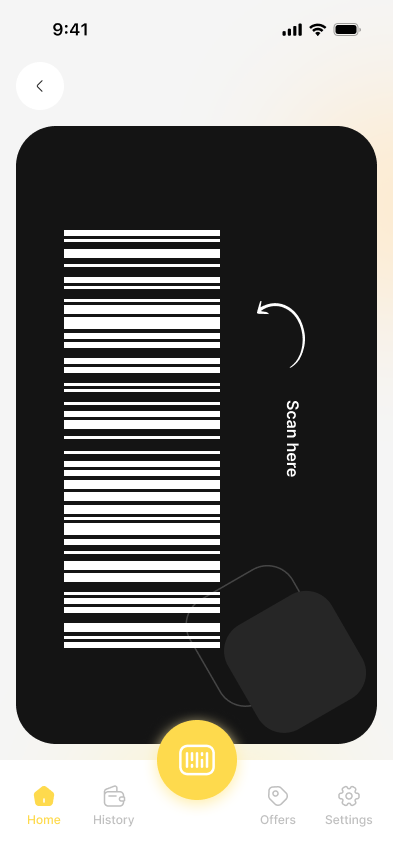
\includegraphics[width=\textwidth]{images/scan_screen.png}
        \caption{Scan Screen}
        \label{fig:scan_screen}
    \end{subfigure}
    \hfill
    \begin{subfigure}[b]{0.32\textwidth}
        \centering
        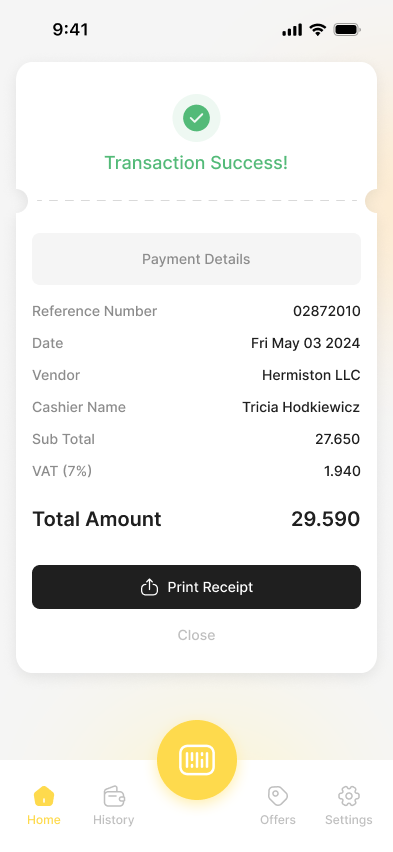
\includegraphics[width=\textwidth]{images/transaction_screen.png}
        \caption{Transaction Screen}
        \label{fig:transaction_screen}
    \end{subfigure}
    \hfill
    \begin{subfigure}[b]{0.32\textwidth}
        \centering
        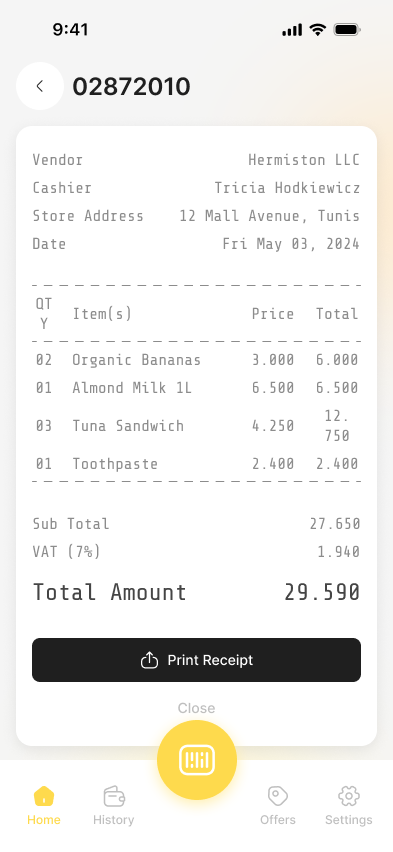
\includegraphics[width=\textwidth]{images/transaction_details_screen.png}
        \caption{Transaction Details Screen}
        \label{fig:transaction_details_screen}
    \end{subfigure}
    \caption{Payment Processing and Transaction Management}
    \label{fig:payment_flow}
\end{figure}

The payment processing workflow prioritizes efficiency and clarity during critical transaction moments. The Scan Screen provides clear visual feedback for QR code scanning with proper camera integration. The Transaction Screen offers immediate confirmation with comprehensive payment details, while the Transaction Details Screen presents a professional receipt format suitable for business documentation—features notably absent in competing solutions.


\begin{figure}[H]
    \centering
    \begin{subfigure}[b]{0.32\textwidth}
        \centering
        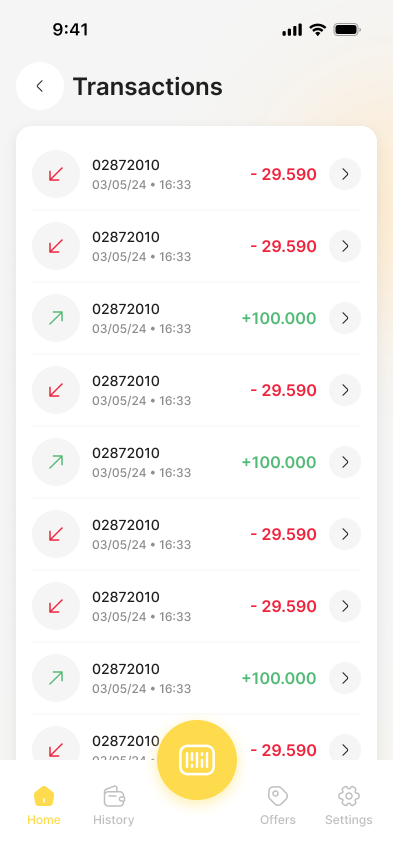
\includegraphics[width=\textwidth]{images/transactions_list_screen.png}
        \caption{Transactions List Screen}
        \label{fig:transactions_list_screen}
    \end{subfigure}
    \hfill
    \begin{subfigure}[b]{0.32\textwidth}
        \centering
        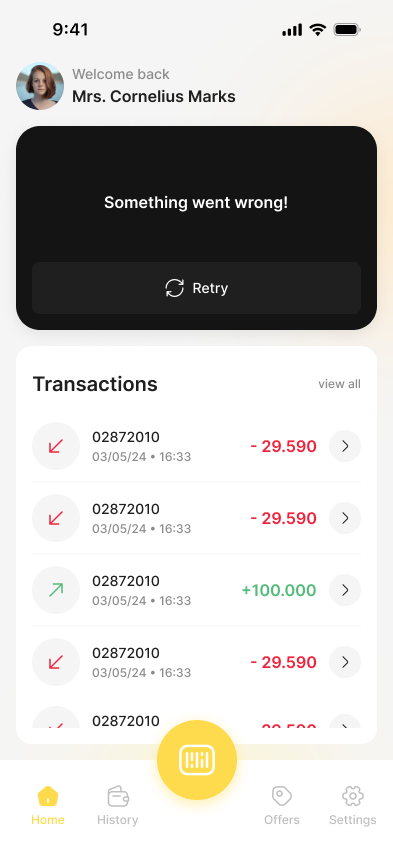
\includegraphics[width=\textwidth]{images/home_screen_wallet_error.png}
        \caption{Home Screen [wallet error]}
        \label{fig:home_screen_wallet_error}
    \end{subfigure}
    \caption{Transaction Management and Error Handling}
    \label{fig:transaction_management}
\end{figure}

The transaction management and error handling interfaces demonstrate robust user experience design. The Transactions List Screen provides comprehensive transaction history with clear visual indicators for different transaction types and easy navigation. The error state handling shows professional error messaging with clear recovery options, ensuring users maintain confidence in the system even during technical difficulties—a critical improvement over the poor error handling observed in existing solutions.

These designs directly address the usability challenges identified in the competitive analysis, providing clear visual feedback, simplified navigation, and efficient task completion paths that are notably absent in existing solutions like Pluxee Tunisia. The interface demonstrates professional financial application standards while maintaining accessibility and ease of use across different user demographics.